\documentclass[12pt,a4paper,oneside]{article}

% -------------------------------------------------------
% Pakete
% -------------------------------------------------------

% Deutsche Sprache und Silbentrennung
\usepackage[ngerman]{babel}

% Zeichenkodierung
\usepackage[T1]{fontenc}
\usepackage[utf8]{inputenc}

% Schriftarten
\usepackage{mathptmx}
\usepackage{courier}
\usepackage{amsmath}

% Farben
\usepackage{xcolor}

% Grafiken einbinden
\usepackage{graphicx}

% Tabellen, Aufzählungen und Quellcode
\usepackage{booktabs}
\usepackage{tabularx}
\usepackage{enumitem}
\usepackage{listings}

% File embedding
\usepackage{embedfile}

% Standardabstände für Listen anpassen
\setlist{itemsep=2pt, topsep=3pt, parsep=2pt}

% Formatierung für Shell-Codeblöcke
\definecolor{codegray}{rgb}{0.96,0.96,0.96}
\definecolor{codeframe}{rgb}{0.85,0.85,0.85}
\lstset{
  backgroundcolor=\color{codegray},
  frame=single,
  framerule=0.5pt,
  rulecolor=\color{codeframe},
  basicstyle=\ttfamily\small,
  breaklines=true,
  showstringspaces=false,
  keepspaces=true
}

% Seitenränder: links 2 cm, rechts 3 cm, oben/unten 2 cm (laut Vorgabe)
\usepackage{geometry}
\geometry{
  a4paper,
  left   = 2cm,
  right  = 3cm,
  top    = 2cm,
  bottom = 2cm,
  includeheadfoot
}

% Zeilenabstand 1,5-zeilig (laut Vorgabe)
\usepackage{setspace}
\onehalfspacing

% Blocksatz ist LaTeX-Standard; Silbentrennhilfen verbessern das Ergebnis
\sloppy

% Kopf- und Fußzeilen mit Seitenzahlen (laut Vorgabe)
\usepackage{fancyhdr}
\pagestyle{fancy}
\fancyhf{}
\fancyfoot[C]{\thepage}
\renewcommand{\headrulewidth}{0pt}

% Hyperlinks im PDF
\usepackage[hidelinks]{hyperref}
\usepackage{xurl}

% including Files
\usepackage{attachfile2}

% Absätze: kein Einzug, dafür vertikaler Abstand
\setlength{\parindent}{0pt}
\setlength{\parskip}{5pt}


% -------------------------------------------------------
% Deckblatt
% -------------------------------------------------------

\title{%
  {\large Netzwerke 1}\\[0.2cm]
  {\huge \textbf{Abgabe 1}}\\[0.4cm]
}

\author{%
  Melvin Lux, Angelina Vorndran\\[0.3cm]
  {\normalsize Bachelor Informatik, 3. Semester}\\[0.2cm]
  {\normalsize Fakult\"at Informatik und Mathematik}\\[0.6cm]
  
\includegraphics[height=2cm]{./images/HM_Schriftzug_Logo_rot_RGB.pdf}%
}

\date{M\"unchen, \today}


% -------------------------------------------------------
% Dokument
% -------------------------------------------------------

\begin{document}

% ---------- Deckblatt ----------
\pagenumbering{alph}
\maketitle
\thispagestyle{empty}
\newpage

% ---------- Beginn der Seitennummerierung ----------
\pagenumbering{arabic}

\section{Blatt 1}

    \subsection*{Aufgabe 1.1: Netzwerk-Traces mit Wireshark}

        \subsubsection*{Teilaufgabe a) Aufruf der Webseite www.cs.hm.edu im Browser}
            \begin{itemize}
                \item \textbf{Beobachtete Protokolle:} DNS, TCP, UDP, TLSv1.3, QUIC
                \item \textbf{Ablauf \& Beschreibung:}
                \begin{enumerate}
                    \item \textbf{DNS (Domain Name System):} Löst den Domainnamen \texttt{www.cs.hm.edu} in die zugehörige IP-Adresse auf (typischerweise über UDP).
                    \item \textbf{TCP / UDP:} Transportprotokolle für den Verbindungsaufbau und die Datenübertragung.
                    \item \textbf{TLSv1.3 / QUIC:} Sichere, verschlüsselte Protokolle zur Übertragung von HTTPS-Webinhalten. QUIC setzt dabei auf UDP auf und kombiniert Verbindungsaufbau sowie Verschlüsselung.
                \end{enumerate}
            \end{itemize}


        \subsubsection*{Teilaufgabe b) Ping auf www.google.com}
            \begin{itemize}
                \item \textbf{Beobachtete Protokolle:} DNS, ICMP / ICMPv6
                \item \textbf{Antwortende IP-Adresse:} \texttt{142.251.153.119}
                \item \textbf{Ablauf \& Beschreibung:}
                \begin{enumerate}
                    \item \textbf{DNS:} Ermittelt die IP-Adresse von \texttt{www.google.com}.
                    \item \textbf{ICMP (Internet Control Message Protocol):} Sendet \textit{Echo Request}-Pakete an die Ziel-IP. Der Rechner antwortet mit \textit{Echo Reply}-Paketen zur Diagnose der Erreichbarkeit und Latenz.
                \end{enumerate}
            \end{itemize}

        \subsubsection*{Teilaufgabe c) FTP-Verzeichnisanzeige (ftp.slackware.com)}
            \begin{itemize}
                \item \textbf{Beobachtete Protokolle:} DNS, TCP, FTP
                \item \textbf{Anmeldedaten (Anonymous-FTP):}
                \begin{itemize}
                    \item Benutzername: \texttt{ftp} oder \texttt{anonymous}
                    \item Passwort: z.\,B. eine E-Mail-Adresse wie \texttt{ftp@melvinlux.de}
                \end{itemize}
                \item \textbf{Erzielte Datenrate:} ca. $11{,}59~\text{MiB/s}$
                \item \textbf{Sicherheitsproblem von FTP:} FTP überträgt Steuerdaten (einschließlich Benutzername und Passwort im Klartext) sowie alle Nutzdaten unverschlüsselt. Ein Angreifer im selben Netzwerk kann diese sensiblen Daten problemlos über Wireshark mitlesen.
            \end{itemize}

        \subsubsection*{Einordnung der Protokolle in die Schichten (OSI-Modell)}

            \begin{table}[h!]
                \centering
                \renewcommand{\arraystretch}{1.15}
                \begin{tabularx}{\textwidth}{l l X}
                \toprule
                \textbf{Protokoll} & \textbf{Schicht im OSI-Modell} & \textbf{Bezeichnung der Schicht} \\
                \midrule
                ARP & Schicht 2 / 3 & Data Link / Network \\
                ICMP & Schicht 3 & Network \\
                TCP / UDP & Schicht 4 & Transport \\
                TLSv1.3 & Schicht 5 & Session \\
                QUIC & Schicht 5 + 6 & Session \& Presentation \\
                DNS, FTP, NTP & Schicht 7 & Application \\
                \bottomrule
                \end{tabularx}
                \caption{Einordnung der beobachteten Netzwerkprotokolle in das OSI-Referenzmodell.}
            \end{table}

    \subsection*{Aufgabe 1.2: Netzwerkkommunikation ganz ohne Netzwerkprogrammierung}

        \subsubsection*{1. Datei von Client zu Server senden}
            \begin{itemize}
                \item \textbf{Server-Seite:}
                \begin{lstlisting}
nc -k -l 4711 > received.txt
                \end{lstlisting}
            \textbf{Erklärung:} Der Server lauscht auf Port 4711 (\texttt{-l}), bleibt nach Verbindungsende aktiv (\texttt{-k}) und leitet alle eingehenden Daten in die Datei \texttt{received.txt} um (\texttt{>}).

            \item \textbf{Client-Seite:}
                \begin{lstlisting}
cat test.txt | nc localhost 4711
                \end{lstlisting}
            \textbf{Erklärung:} Der Inhalt der Datei \texttt{test.txt} wird über die Pipe (\texttt{|}) an den Client \texttt{nc} übergeben und an den lokalen Port 4711 gesendet.
        \end{itemize}

    \subsubsection*{2. Netzwerkdienst zur Umwandlung von Texten}
        \begin{itemize}
            \item \textbf{Server-Seite:}
            \begin{lstlisting}
nc -l 4711 < pipe | sed -u 's/Vorlesung/Party/g' > pipe
            \end{lstlisting}
            \textbf{Erklärung:}
            \begin{enumerate}
                \item \texttt{mkfifo pipe}: Erstellt eine benannte Pipeline (Named Pipe), um eine Rückkopplung/Schleife für Daten zu ermöglichen.
                \item \texttt{nc -l 4711 < pipe}: Liest die verarbeitete Antwort aus der Named Pipe und schickt sie zurück an den Client.
                \item \texttt{| sed -u 's/Vorlesung/Party/g'}: Der Stream wird durch \texttt{sed} verarbeitet. Jedes Vorkommen von \texttt{"Vorlesung"} wird global (\texttt{/g}) durch \texttt{"Party"} ersetzt. Die Option \texttt{-u} (\textit{unbuffered}) stellt sicher, dass der Text sofort ohne Pufferung ausgegeben wird.
                \item \texttt{> pipe}: Schreibt das Ergebnis zurück in die Named Pipe.
            \end{enumerate}

            \item \textbf{Client-Seite:}
            \begin{lstlisting}
nc localhost 4711
            \end{lstlisting}
            \textbf{Erklärung:} Baut eine interaktive Verbindung zum Dienst auf Port 4711 auf. Nach der Eingabe von z.\,B. \texttt{Ist morgen Vorlesung?} empfängt der Client die Antwort \texttt{Ist morgen Party?}.
        \end{itemize}
    
\section{Blatt 2}

    \subsection{Aufgabe 2.1}
        \subsubsection{a}
        \begin{center}
            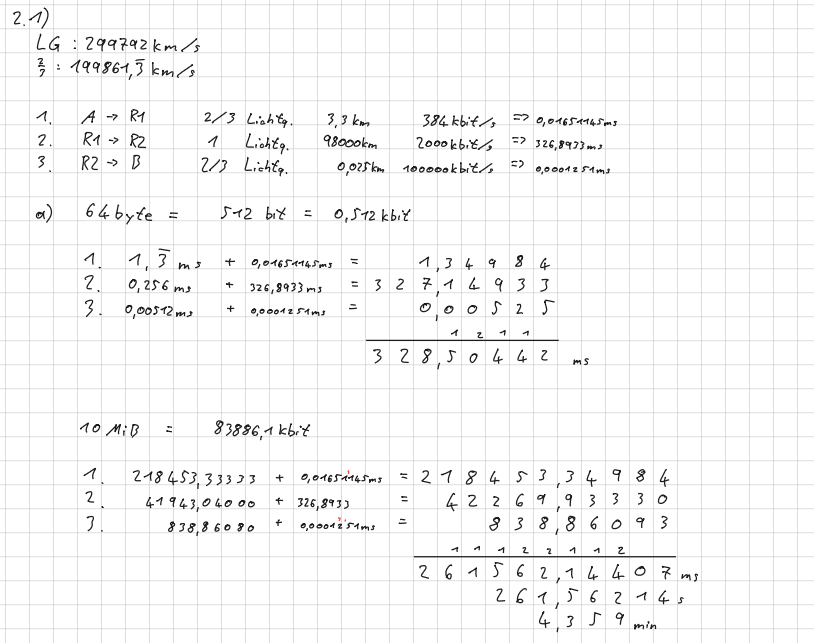
\includegraphics[width=\textwidth]{images/Blatt-2/Aufgabe_2-1-a.png}
        \end{center}
            
        \subsubsection{b}

        \subsubsection{c}
            Wenn man eine der Variablen verändern könnte würden wir die Übertragungsrate vom 1. Schritt (A->R1) erhöhen um die dortigen Zeiten drastisch zu erhöhen.

        \subsubsection{d}
            \begin{center}
                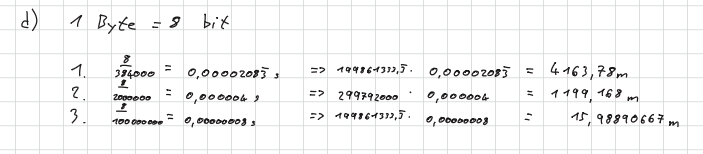
\includegraphics[width=\textwidth]{images/Blatt-2/Aufgabe_2-1-d.png}
            \end{center}

        \subsubsection{e}

    \subsection{Aufgabe 2.2}
        \subsubsection{a}
            Das Internet-Schichtenmodell unterscheidet sich vom ISO/OSI-Schichtenmodell hauptsächlich an 2 Stellen, indem es einige Schichten zusammenfasst:
            \begin{itemize}
                \item 1. Verbindungsschicht -> Bitübertragungsschicht \& Sicherungsschicht
                \item 2. Anwendungsschicht -> Kommunikationssteuerung \& Darstellungsschicht \& Anwendungsschicht
            \end{itemize}
            Im Allgemeinen lässt sich sagen, dass das Internet-Schichtenmodell das ISO/OSI-Schichtenmodell simplifiziert und für den Endanwender unnötige Schichten zusammenfasst.

        \subsubsection{b}
            Funktionalität wird im Internet immer auf der höchstmöglichen Schicht realisiert, um keine neue Hardware in der Infrastruktur zu benötigen, die Netzneutralität nicht zu gefährden und um weitere Kosten durch den Netzbetreiber vermeiden zu können.

        \subsubsection{c}
            Nein. Ein zuverlässiges Schicht-2-Protokoll garantiert die korrekte Übertragung nur zwischen zwei direkt verbundenen Knoten, also pro Teilstrecke. Auf dem Weg zwischen den Endsystemen können Pakete trotzdem verloren gehen (z. B. durch überlaufende Router-Puffer), verfälscht werden (Fehler im Router nach der Link-Prüfung), dupliziert werden oder in falscher Reihenfolge ankommen. Diese Fehler werden auf Schicht 2 nicht erkannt. Zuverlässigkeit muss daher Ende-zu-Ende gewährleistet werden, also im Transportprotokoll (TCP) oder in der Anwendung. UDP bietet das nicht. Der gesparte Overhead würde die Zuverlässigkeit gefährden.

    \subsection{Aufgabe 2.3}
        \subsubsection{HelloServer}
            Der Vollständige Code ist in \textattachfile[description={Doppelklick zum Download}]{socket/src/main/java/HelloServer.java}{HelloServer.java} zu finden.

        \subsubsection{FreeDiskSpaceClient}
            Der Vollständige Code ist in \textattachfile[description={Doppelklick zum Download}]{socket/src/main/java/FreeDiskSpaceClient.java}{FreeDiskSpaceClient.java} zu finden.

\section{Blatt 3}
    \subsection{3.1}
        \subsubsection{a}
            $https://cs.hm.edu/aktuelles/news/news_detailseite_133888.de.html$
        \subsubsection{b}
            Ja, damit kann umgegangen werden, da im Header "Accept-Encoding" gzip enthalten ist.
        \subsubsection{c}
            Es wird eine persistente Verbindung erwartet, da der Header "Connection" den Wert keep-alive hat.
        \subsubsection{d}
            Wenn der Header "If-None-Match" der Server würde ausschließlich Datein zurückgeben die den ETag "ddnenj89j4jf8ejf8juw37EEjh8Suf3" nicht besitzen, dann würde auch der Code 200 gesendet werden, wenn eine solche Datei existiert bekommen wir 304 "Not Modified" zurück.
        \subsubsection{e}
            Der Server kann mit 2 Möglichkeiten antworten:
            \begin{itemize}
                \item{200 --- OK} \begin{center} 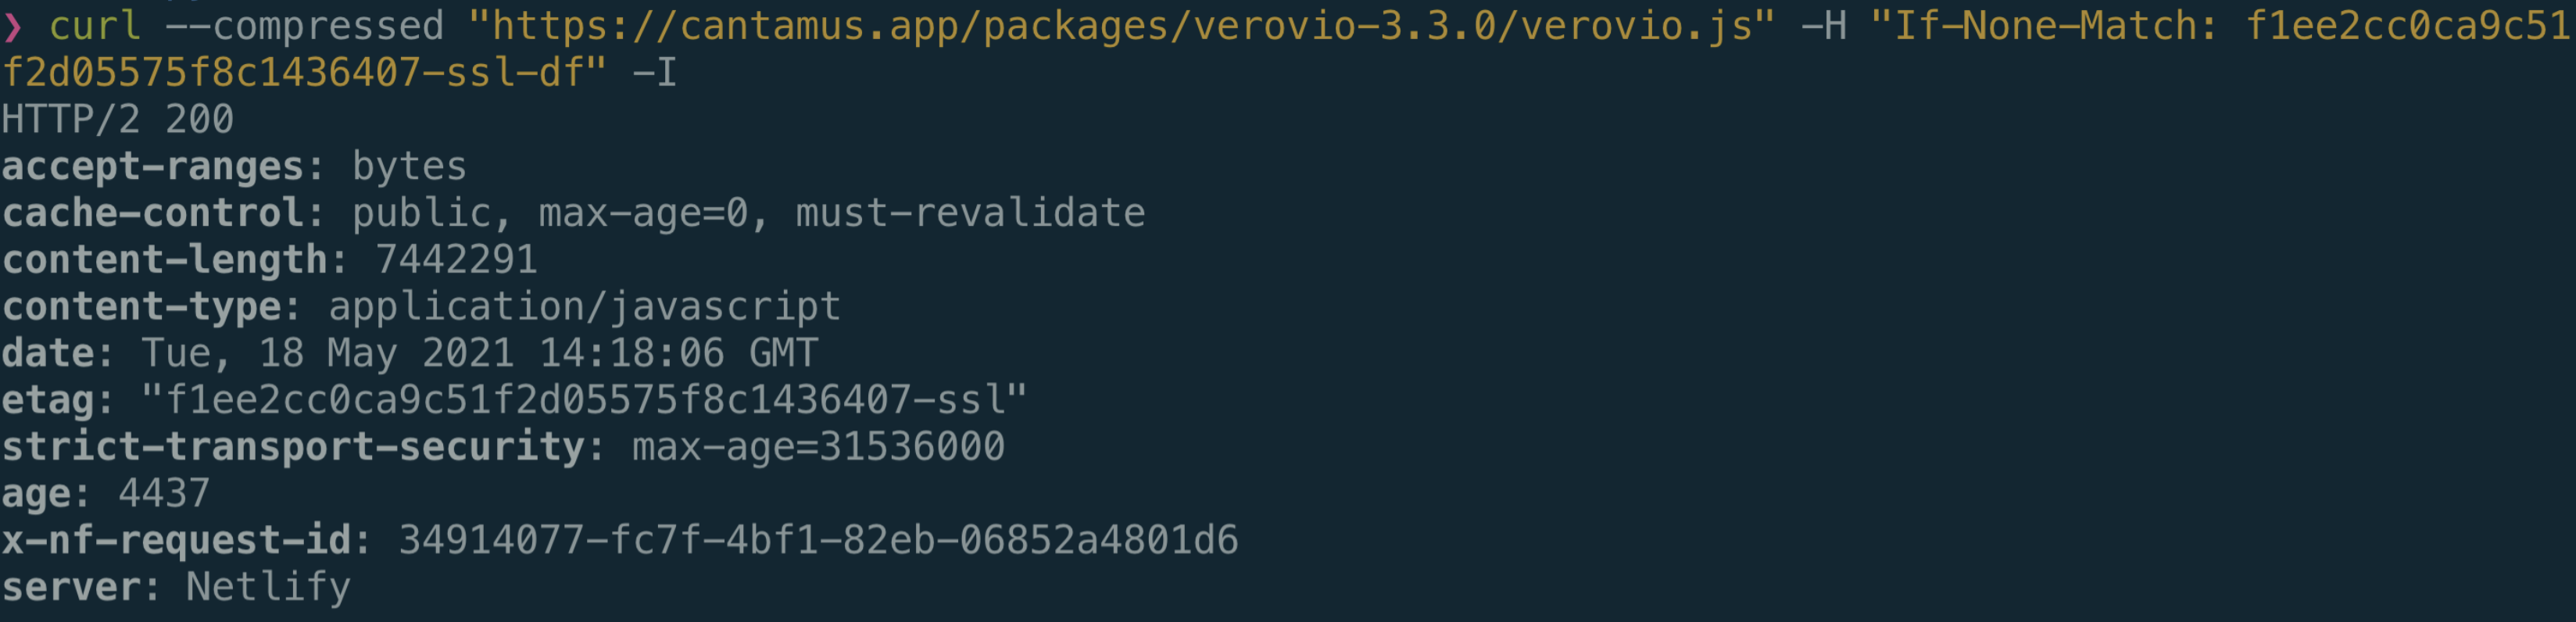
\includegraphics[width=\textwidth]{images/Blatt-3/task_3-1-e-200.png} \end{center}
                \item{304 --- Not Modified} \begin{center} 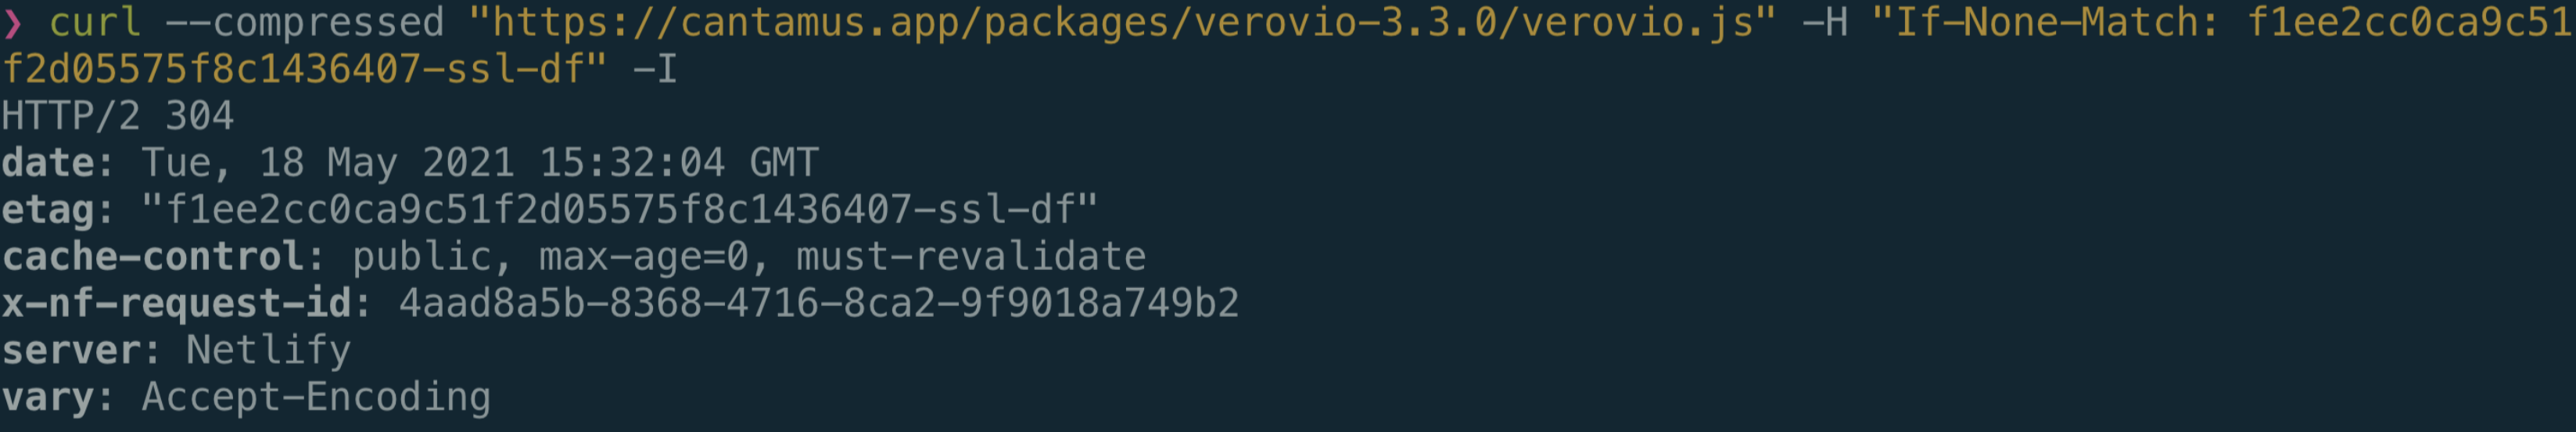
\includegraphics[width=\textwidth]{images/Blatt-3/task_3-1-e-304.png} \end{center}
            \end{itemize}
    \subsection{3.2}
            

    \subsection{3.3}
        \subsubsection{a}
            Es werden die Datein aus dem Ordner angezeigt, indem der Befehl ausgeführt wurde, hier das Homeverzeichnis.
            \begin{center}
                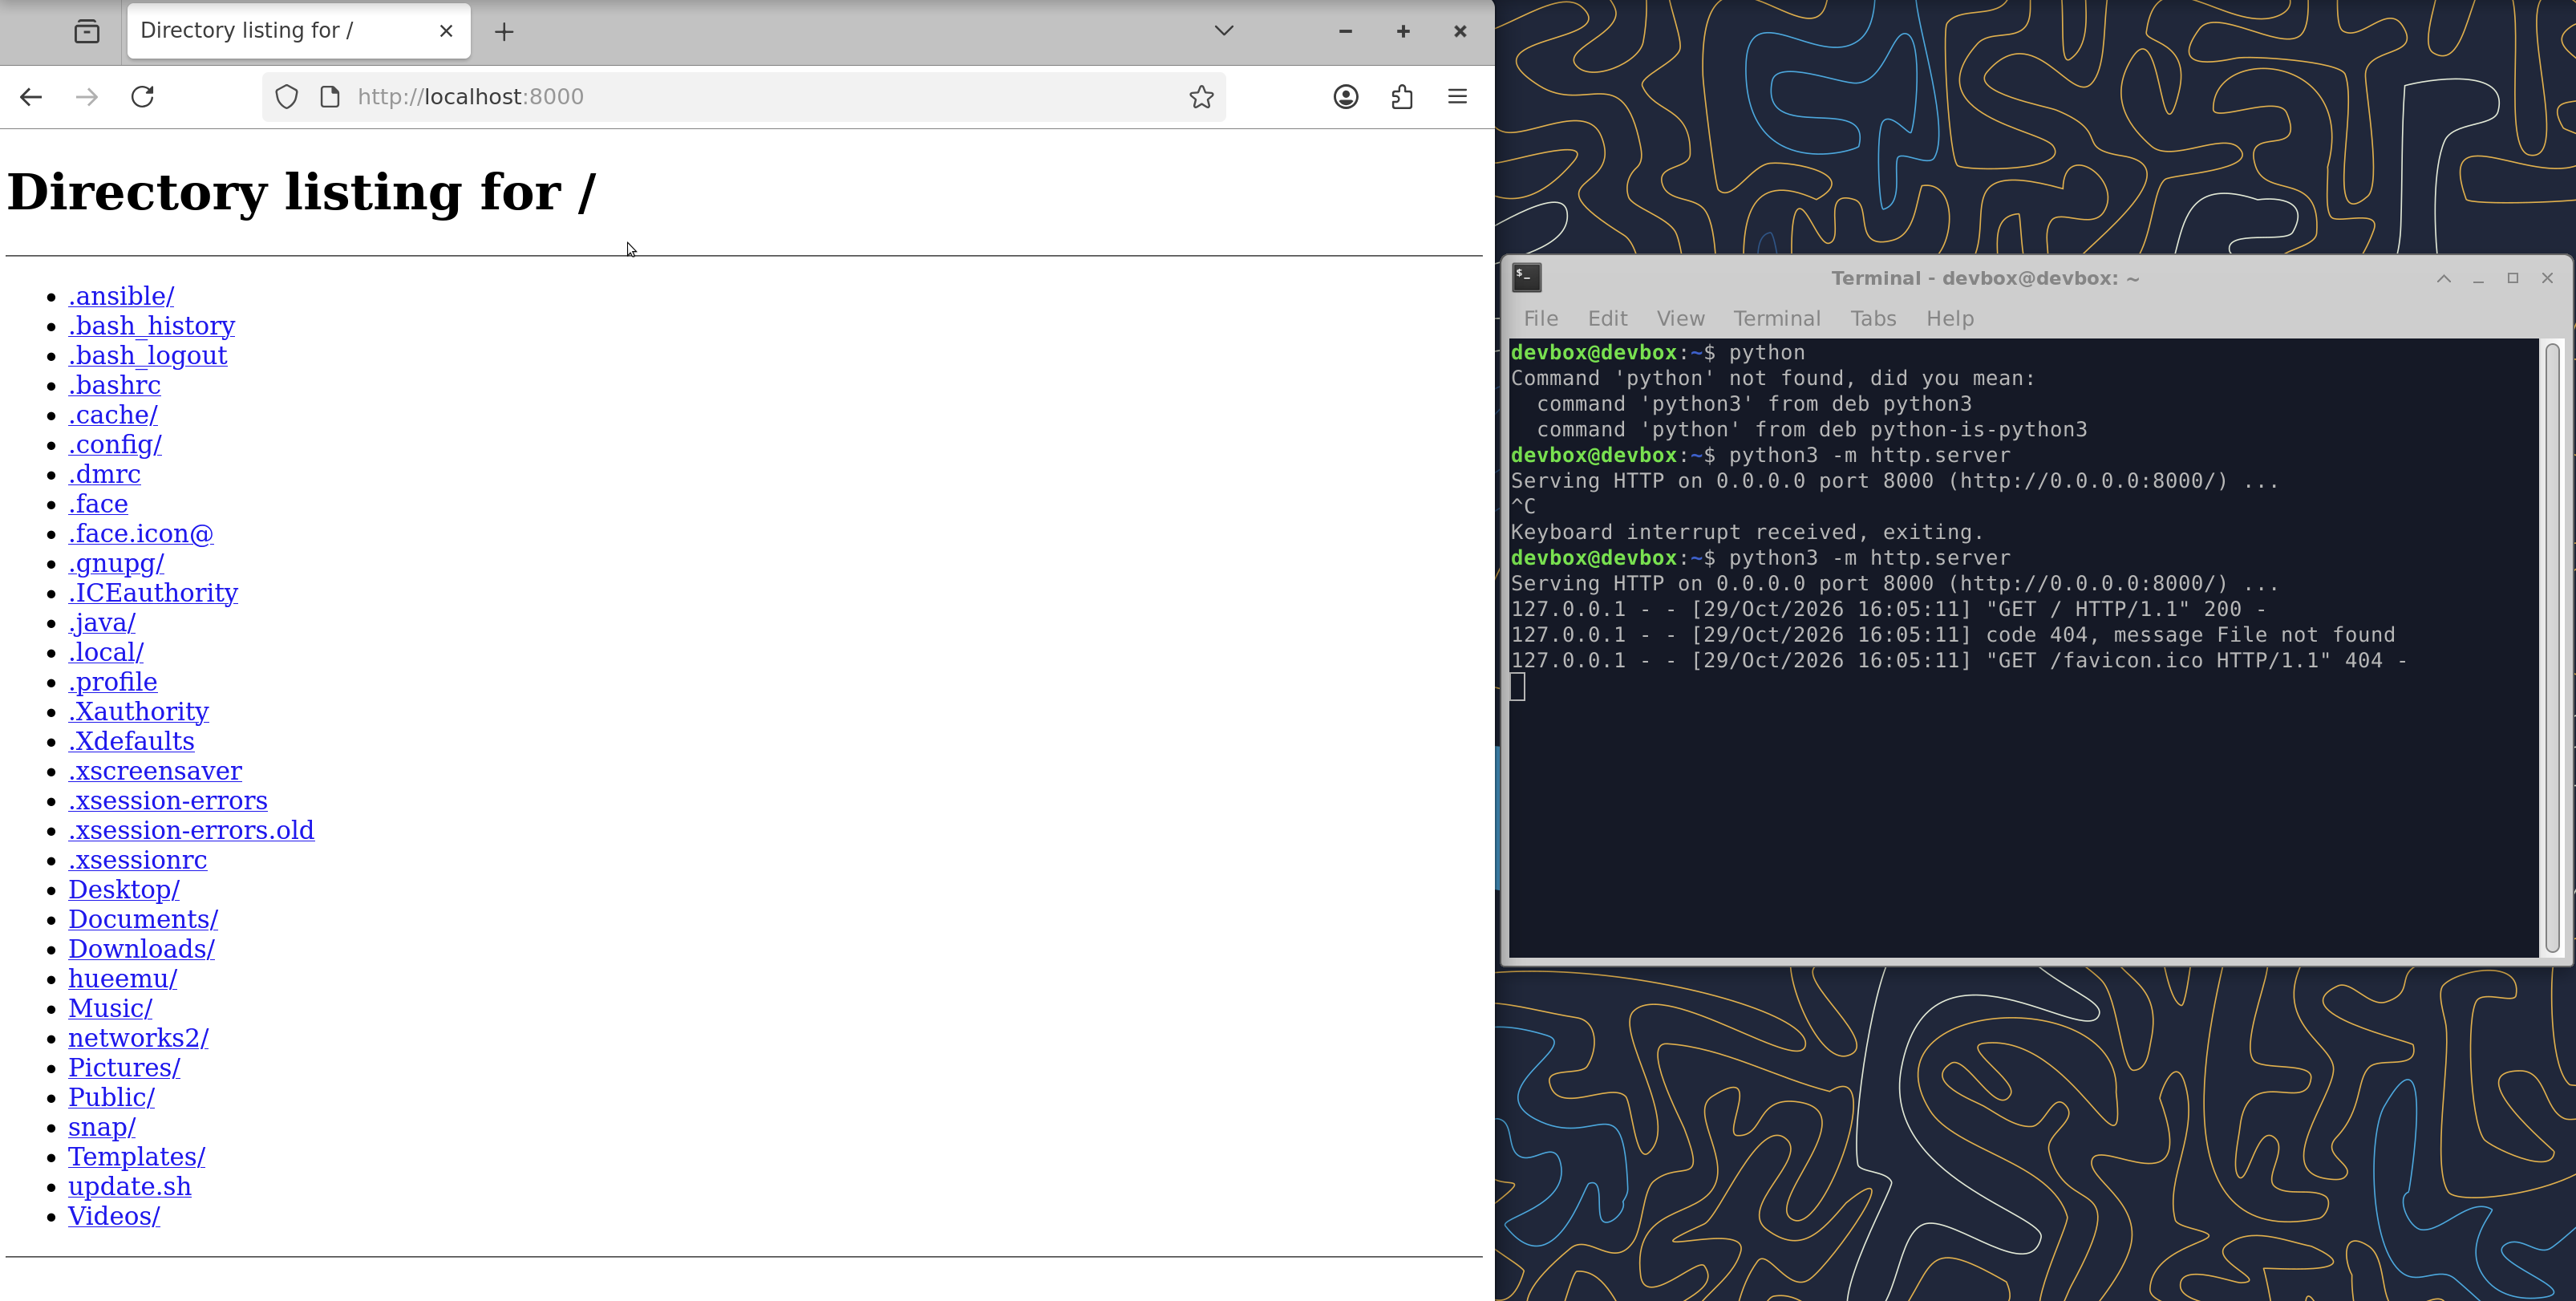
\includegraphics[width=\textwidth]{images/Blatt-3/task_3-2-a.png}
            \end{center}

        \subsubsection{b}
            \begin{center}
                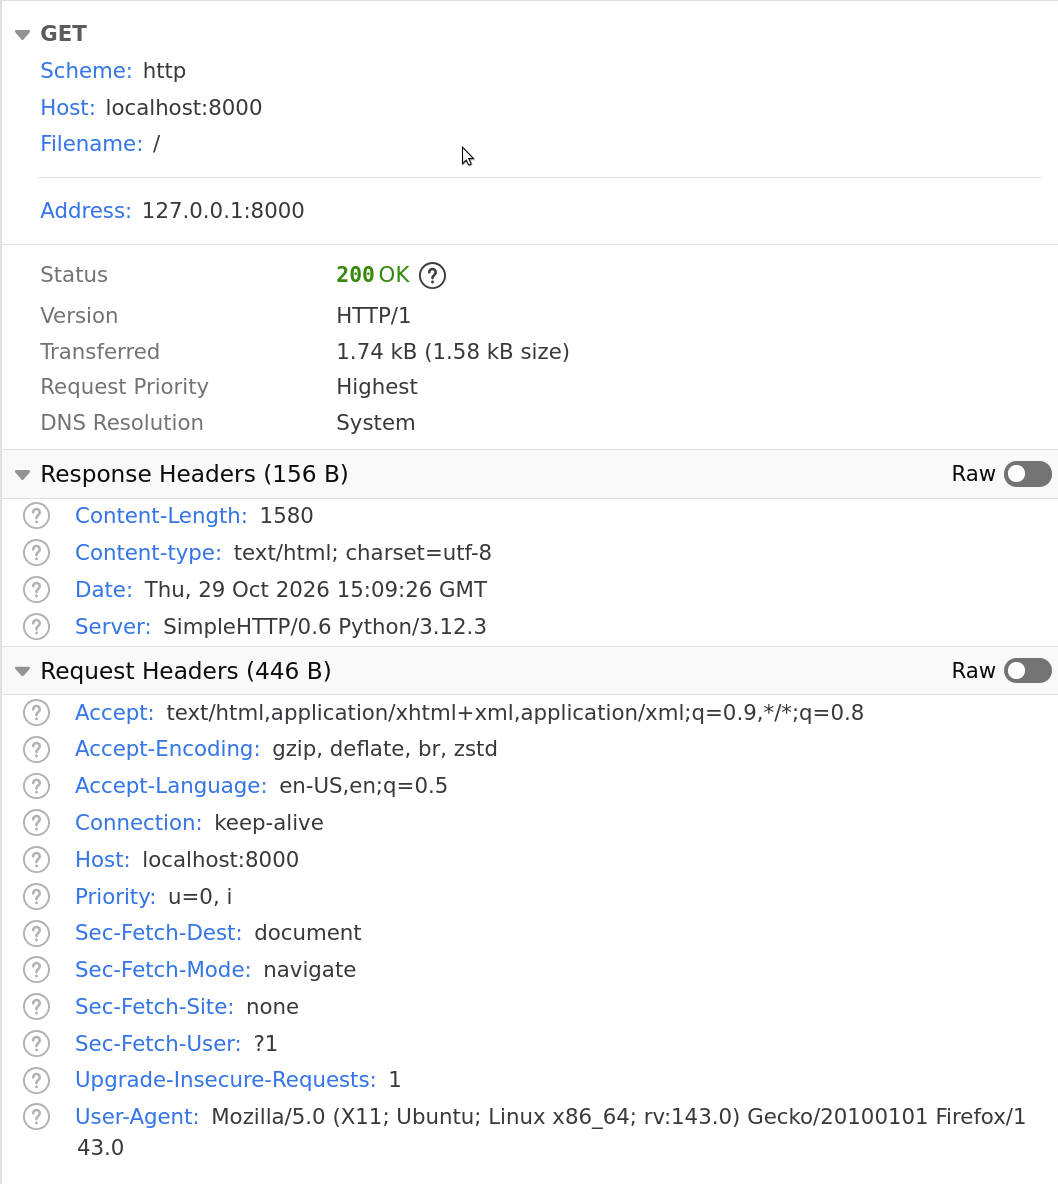
\includegraphics[width=\textwidth]{images/Blatt-3/task_3-2-b.png}
            \end{center}

        \subsubsection{c}
    \subsection{3.4}
//TODO: Bild hinzufügen
    Der Code liegt in der Klasse HelloServer
    \subsection{3.5}
        \subsubsection{c}
            \begin{center}
                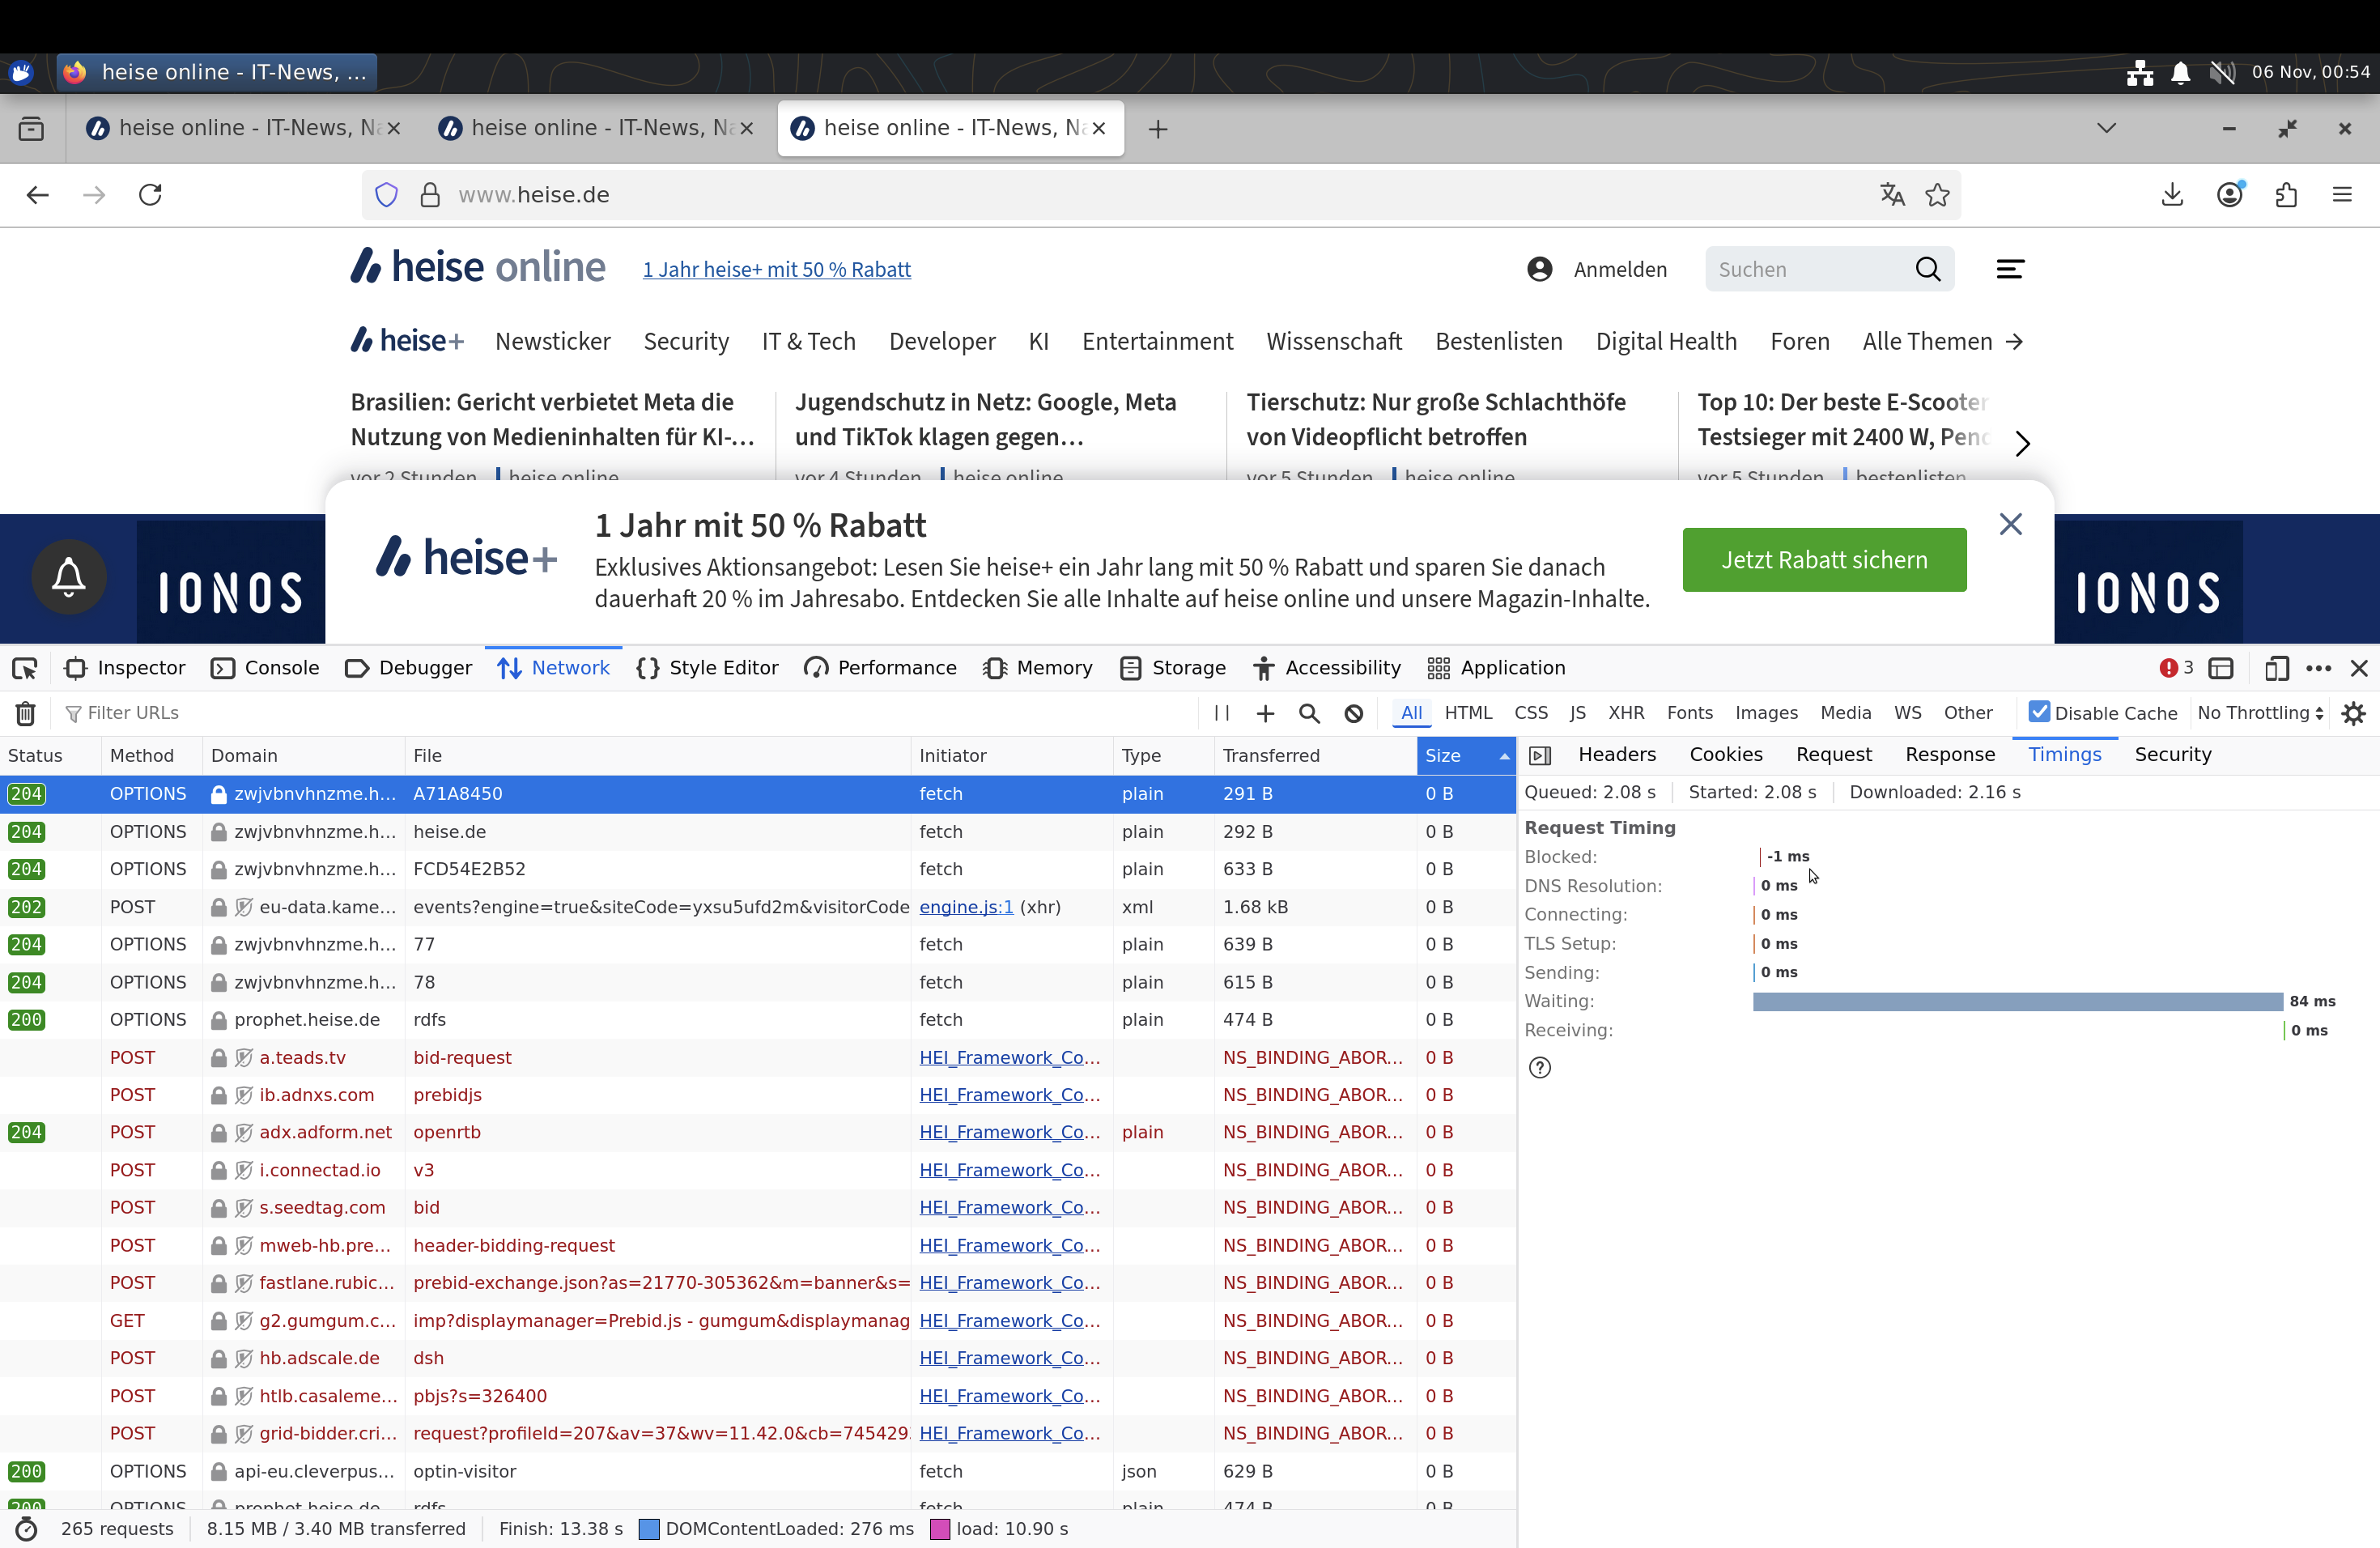
\includegraphics[width=\textwidth]{images/Blatt-3/task_3-5-c}
            \end{center}
        Wie im Bild zu erkennen ist, wurden 265 Objekte geladen, was insgesamt 13.38s gedauert hat.
        Das kleinste Objekt ist 0 Bytes groß mit einer Zeit von 84 ms. Der TCP Verbindungsaufbau hat 0 ms gedauert.
        \subsubsection{d}
        Die Daten werden von Wireshark mit Hilfe von ip.addr == 193.99.144.85 gefiltert. Die IP von der Webseite heise.de wurde davor herausgefunden.
        Folgende Protokolle werden bei heise.de angezeigt: IPv4 auf der Netzwerkschicht, TCP auf der Transportschicht und TLSv1.3 auf der Anwendungsschicht
        Für google.com werden hingegen IPv4 auf der Netzwerkschicht, UDP auf der Transportschicht und QUIC auf der Anwendungsschicht angezeigt.
        Der wesentliche Unterschied besteht darin, dass heise.de TCP nutzt, welches einen zeitaufwendigen Handshake für den Verbindungsaufbau und die Verschlüsselung benötigt.
        Google.com verwendet das QUIC-Protokoll über das verbindungslose UDP, welches die Verschlüsselung direkt integriert.

\end{document}
